\documentclass[aspectratio=169,x11names]{beamer}
\usetheme{Pittsburgh}
\usepackage{xcolor}
\usepackage[utf8]{inputenc}
\usepackage[german]{babel}
\usepackage{amsmath}
\usepackage{amsfonts}
\usepackage{amssymb}
\usepackage{graphicx}
\usepackage{multicol}
\usepackage{wrapfig}
\usepackage{hyperref}
\usepackage{tikz}
\usepackage{upgreek}
\usetikzlibrary{shapes,arrows,chains}

\author{Jonas Betzendahl}
\title{Hello, I'm your Edge Case}

\beamertemplatenavigationsymbolsempty 

%src: https://tex.stackexchange.com/questions/34921/how-to-overlap-images-in-a-beamer-slide
\def\Put(#1,#2)#3{\leavevmode\makebox(0,0){\put(#1,#2){#3}}}

\definecolor{darkgray}{rgb}{0.2,0.2,0.2}
\definecolor{darkred}{rgb}{0.25,0,0}
\definecolor{darkgreen}{rgb}{0,0.25,0}

\begin{document}

\setbeamercolor{background canvas}{bg=darkgray}

\setbeamercolor{normal text}{fg=white}
\usebeamercolor[fg]{normal text}

\setbeamercolor{titlelike}{fg=white}
\usebeamercolor[fg]{titlelike}

%------------------------------------------------------------------------------------
\section{Introduction}

\begin{frame}
\begin{center}
\vfill
\huge ``Hello, I'm your Edge Case!''
\normalsize 
\smallskip
\smallskip

or\\
``No, seriously! How \emph{do} you ask someone\\ for their gender on the internet?!''

\bigskip\bigskip

\large $\uplambda$Totoro\\
36c3, Chaos West
\bigskip\bigskip

\href{https://twitter.com/lambdatotoro}{
\includegraphics[scale=0.125]{images/twitter_logo.png}}
\href{https://chaos.social/@lambdatotoro}{\includegraphics[scale=0.125]{images/mastodon_logo.png}}
\href{https://github.com/lambdaTotoro}{
\includegraphics[scale=0.125]{images/github_logo.png}}
\href{https://whispeer.de/en/user/jbetzend}{
\includegraphics[scale=0.125]{images/whispeer_logo.png}}

\texttt{@lambdaTotoro (@chaos.social)}
\end{center}
\end{frame}

\begin{frame}
\frametitle{Who am I?}

\begin{minipage}{0.5\textwidth}
Hello! I am $\uplambda$Totoro. Good to see you!\\
I am many things, among them \dots
\medskip

\begin{itemize}
\item\dots nonbinary.
\item\dots a M.Sc. in Intelligent Systems
\item\dots a CS PhD student @ FAU Erlangen
\item\dots a science communicator
\item\dots not a doctor / psychologist
\end{itemize}
\end{minipage}%
\begin{minipage}{0.5\textwidth}
\begin{center}

\includegraphics[width=0.8\textwidth,keepaspectratio]{images/pigeon_jonas} 
\end{center}
\end{minipage}
\end{frame}

\begin{frame}
\frametitle{Who are you?}
\end{frame}

\begin{frame}
\frametitle{What is this talk? (1)}
\large
It's a talk about this:\medskip

\begin{center}
\includegraphics[scale=0.45]{images/Simba_01}
\end{center}
\end{frame}

\begin{frame}
\frametitle{What is this talk? (2)}
\large

This is a talk on forms and about the responsibilities of people who design them. It's a talk about how technology is not politically neutral.

\pause\bigskip

\begin{center}
Content Notes:\\
\emph{Discussion of transmisia, intermisia, involuntary surgery}
\end{center}

\pause\bigskip

I aim for roughtly the following composition:

\begin{itemize}
\item One part Education, ``Humans 201''
\item One part Advice, ``Good form design''
\item One part Fun, ``Hilarious Form Fails''
\end{itemize}
\end{frame}

\begin{frame}
\begin{center}
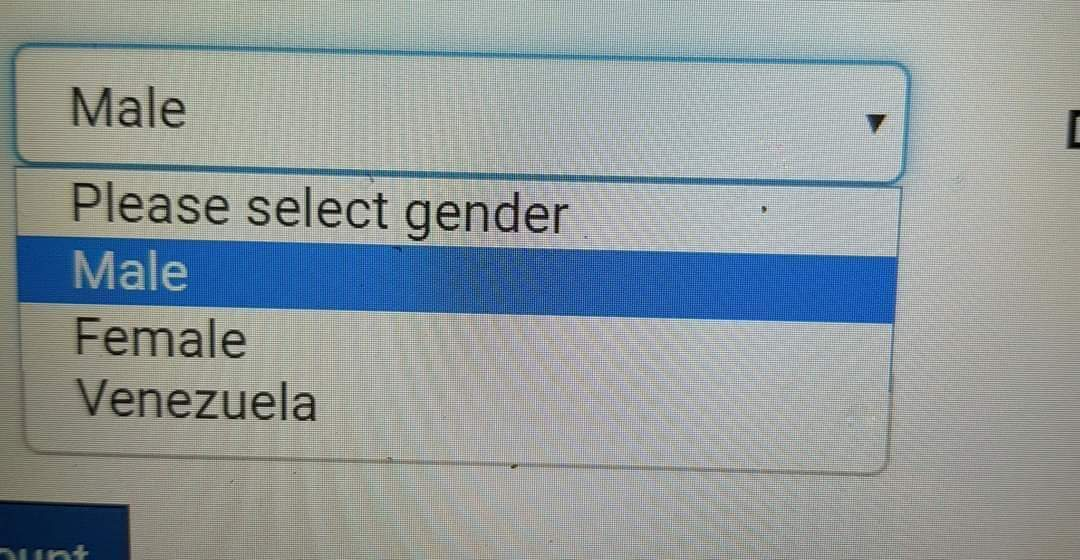
\includegraphics[scale=0.3]{images/ineffyble_01} 
\end{center}
\end{frame}


\begin{frame}
\frametitle{Axioms!}
A few things this talk is \emph{not} an invitation to debate:
\bigskip

\begin{itemize}
\item\emph{Trans people exist.}\\
Trans women are women. Trans men are men. Nonbinary people are nonbinary.
\medskip

\item\emph{Cultural differences exist.}\\
Culture influences almost every aspect of our lives. A way of doing things is not less valid because it is new or strange to you.
\end{itemize}
\bigskip

\huge
\begin{center}
\texttt{><((((*>}
\end{center}

\end{frame}

\begin{frame}
\frametitle{Conclusions, up front!}
\large
The central points of this talk are as follows:\bigskip

\begin{itemize}
\pause\item \textbf{Make the model fit the user and not vice versa!}\\
\emph{All models are wrong, some are useful. Stereotypes aren't!}\medskip
\pause\item \textbf{Humans are moving targets!}\\
\emph{Humans change all the time. Your model will have to change with them!}\medskip
\pause\item \textbf{The empty model makes the fewest mistakes!}\\
\emph{You can't draw wrong conclusions from data you don't collect.}\medskip
\pause\item \textbf{Precision and transparency are key!}\\
\emph{Make sure that both you and your users know what you're using the data for.}
\end{itemize}
\end{frame}

%------------------------------------------------------------------------------------

\section{Edge Cases}

\begin{frame}
\begin{center}
\huge
Hello!\\
I'm your edge case!\medskip\large

(stories about making the model fit you)
\end{center}
\end{frame}

\subsection{More than two genders}

\setbeamercolor{background canvas}{bg=darkred}
\begin{frame}
\begin{center}
\huge
There's only two genders...
\end{center}
\end{frame}
\setbeamercolor{background canvas}{bg=darkgray}

\begin{frame}
\begin{center}
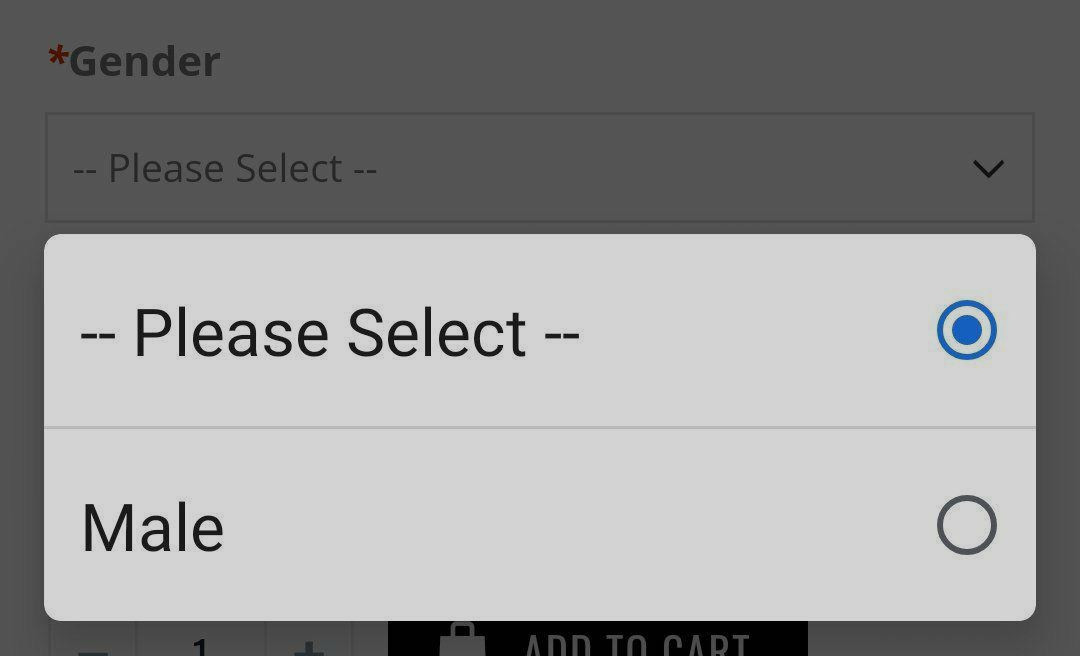
\includegraphics[scale=0.3]{images/please_select_male.jpg} 
\end{center}
\end{frame}

\begin{frame}
\frametitle{Legal Recognition for Nonbinary People}
\end{frame}

\setbeamercolor{background canvas}{bg=darkgreen}
\begin{frame}
\begin{center}
\huge
There's \emph{more} than two genders!\medskip

\Large
$\Rightarrow$ \emph{Don't store gender in a Boolean.}
\end{center}
\end{frame}
\setbeamercolor{background canvas}{bg=darkgray}


\setbeamercolor{background canvas}{bg=darkred}
\begin{frame}
\begin{center}
\huge
Okay, three! There's only three genders!
\end{center}
\end{frame}
\setbeamercolor{background canvas}{bg=darkgray}

\begin{frame}
\begin{center}
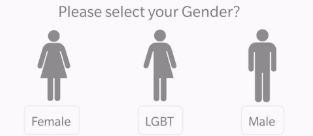
\includegraphics[height=0.6\textheight,keepaspectratio]{images/gender_m_lgbt_f.jpg} 
\bigskip\Large

(LGBT = Lesbian, Gay, Bi, Trans $\notin$ Genders)
\end{center}
\end{frame}

\begin{frame}
\begin{center}
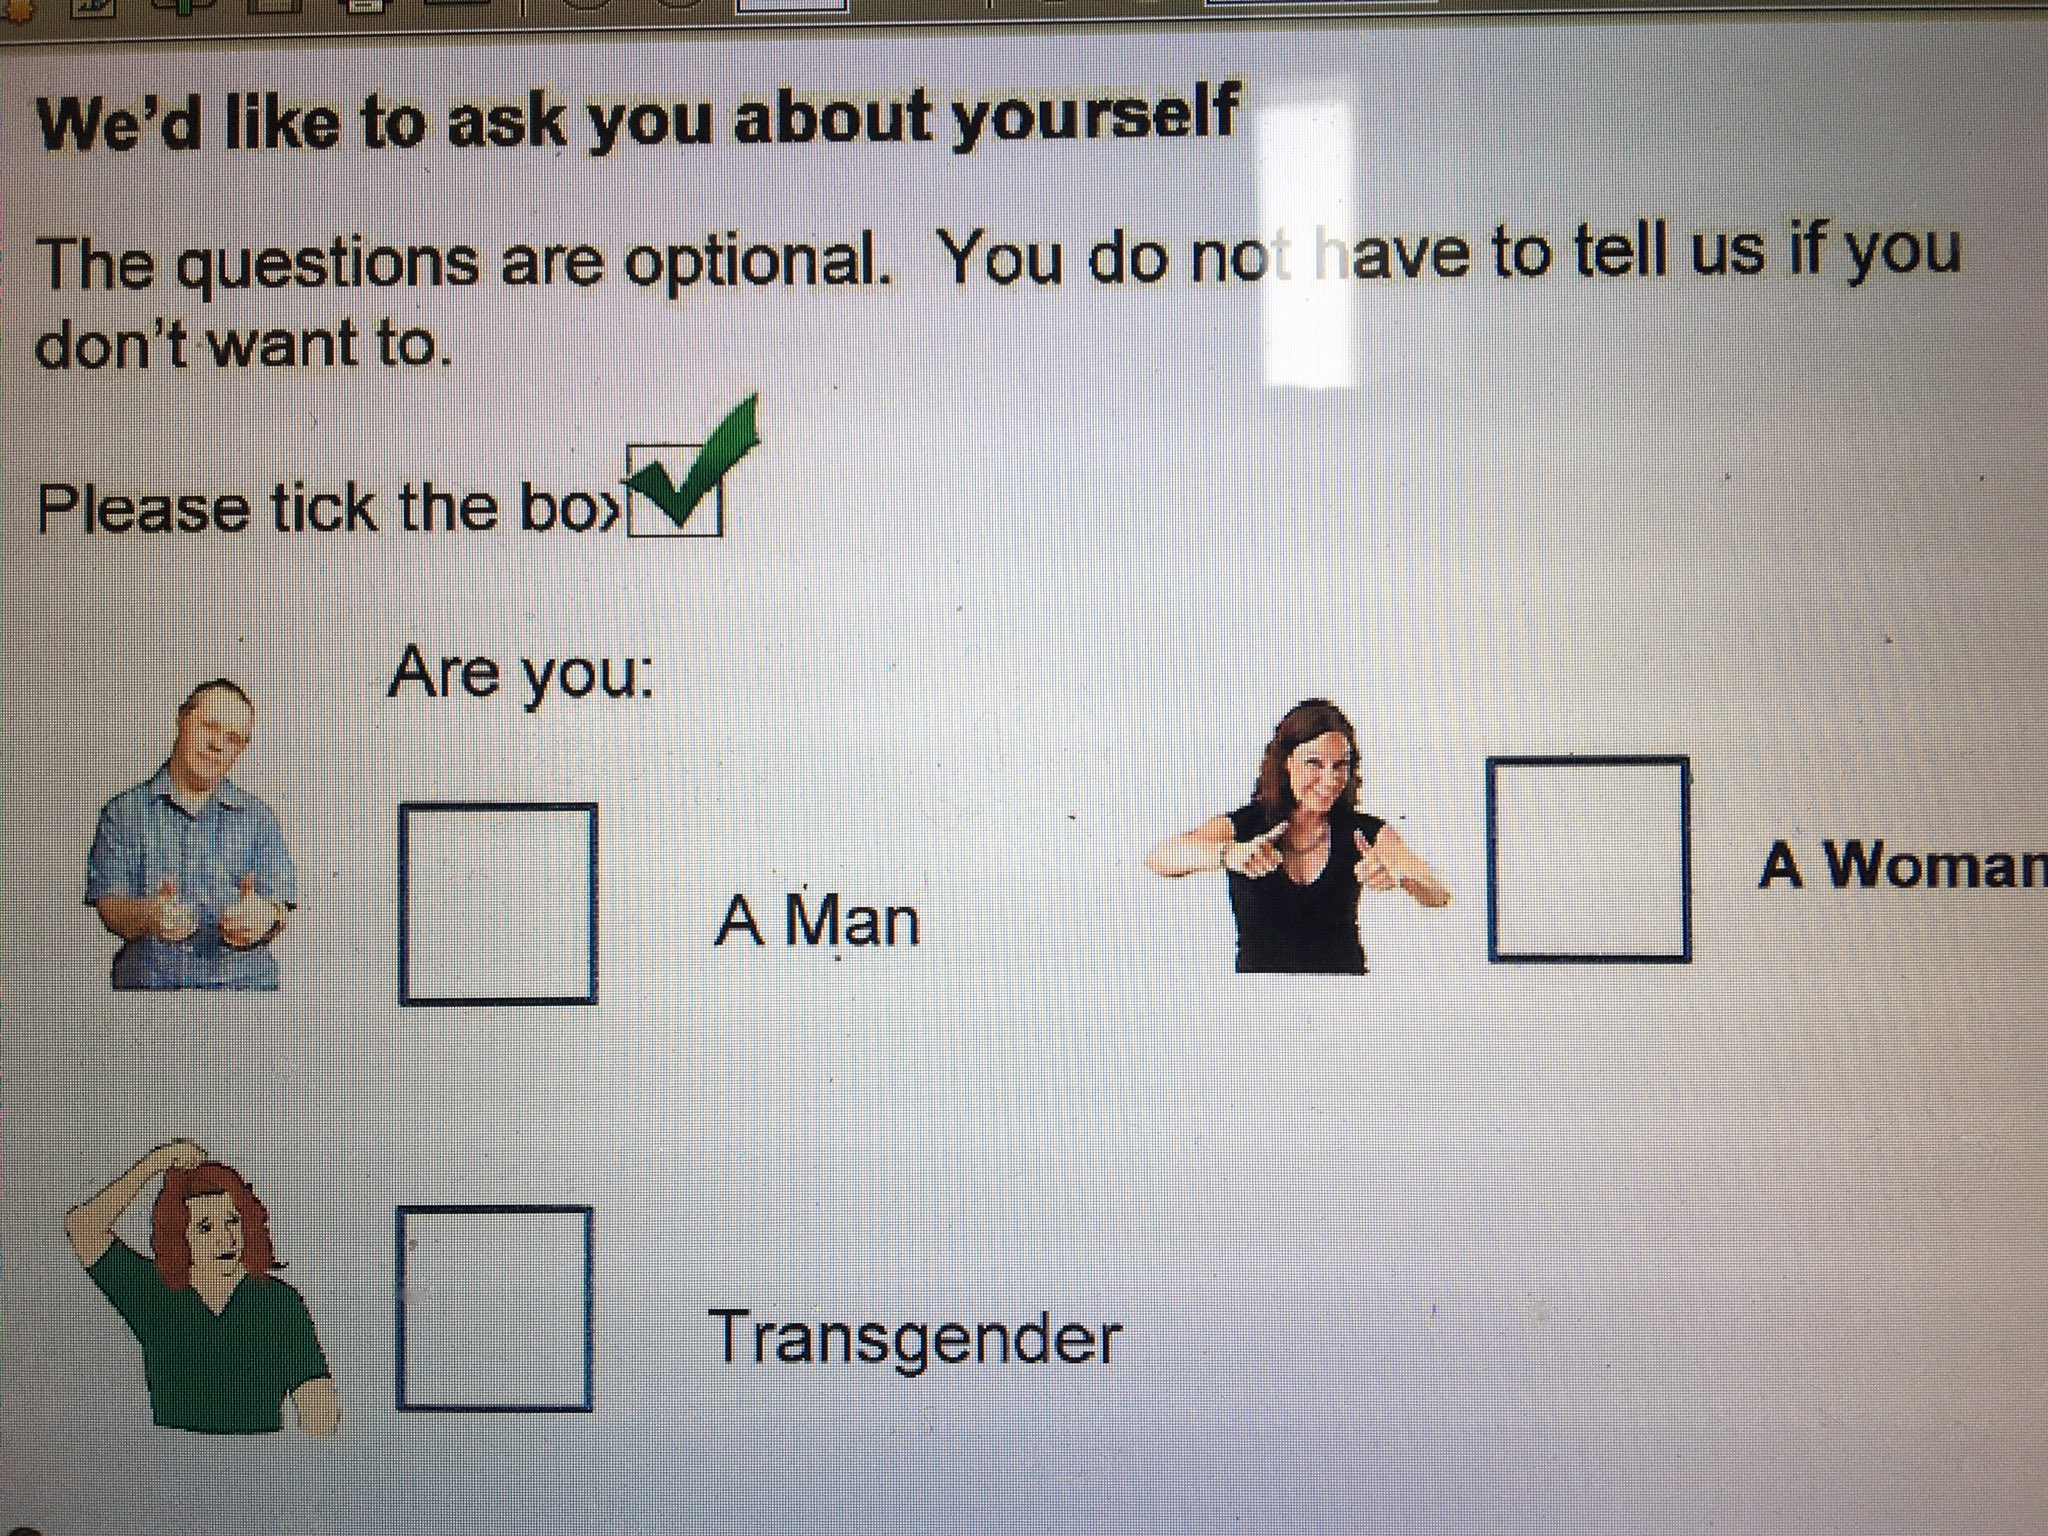
\includegraphics[height=0.75\textheight,keepaspectratio]{images/mftrans.jpg} 
\bigskip\Large

Also, please think about messages you're sending!
\end{center}
\end{frame}

\begin{frame}
\frametitle{Even corporations are catching on...}
\begin{center}

\includegraphics[width=0.9\textwidth,keepaspectratio]{images/tinder_gender.png} 
\end{center}
\pause
\Put(100,00){
\includegraphics[scale=0.5,angle=10]{images/800px-Genderqueer.png}}
\pause
\Put(300,100){
\includegraphics[scale=0.5,angle=-10]{images/800px-Genderfluid.png}}
\pause
\Put(0,150){
\includegraphics[scale=0.5,angle=-5]{images/800px-Agender-4.png}}
\pause
\Put(225,275){
\includegraphics[scale=0.5,angle=-5]{images/800px-Neutrois.png}}
\pause
\Put(25,275){
\includegraphics[scale=0.5,angle=0]{images/800px-Bigender-2.png}}
\pause
\Put(125,200){
\includegraphics[scale=0.5,angle=0]{images/800px-Trigender-4.png}}
\pause
\Put(200,125){
\includegraphics[scale=0.5,angle=0]{images/800px-Polygender.png}}
\pause
\Put(200,0){
\includegraphics[scale=0.5,angle=0]{images/800px-Pangender.png}}
\end{frame}

\setbeamercolor{background canvas}{bg=darkred}
\begin{frame}
\begin{center}
\huge
I see, it's not three either.\\
But however many you just said is enough, right?
\end{center}
\end{frame}
\setbeamercolor{background canvas}{bg=darkgray}

\begin{frame}
\frametitle{Humans are still a Moving Target}
\begin{center}
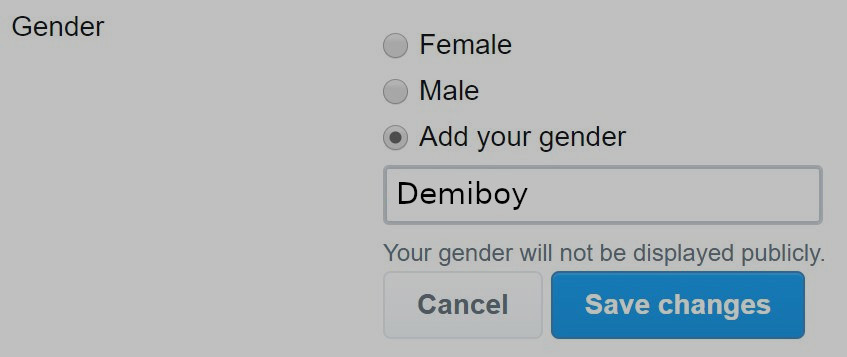
\includegraphics[width=0.9\textwidth,keepaspectratio]{images/statistical_outlier.jpg} 
\medskip

\Large \emph{It's not a statistical outlier if enough people do it\dots}
\end{center}
\end{frame}

\setbeamercolor{background canvas}{bg=darkgreen}
\begin{frame}
\begin{center}
\huge
There's \emph{so many} genders!\medskip

\Large
$\Rightarrow$ \emph{Don't store gender in an enum, either.}
\end{center}
\end{frame}
\setbeamercolor{background canvas}{bg=darkgray}

\subsection{More than two biological sexes}

\setbeamercolor{background canvas}{bg=darkred}
\begin{frame}
\begin{center}
\huge
But there's only two \emph{biological sexes}... right?
\end{center}
\end{frame}
\setbeamercolor{background canvas}{bg=darkgray}

\begin{frame}
\frametitle{Intersex}
\begin{minipage}{0.475\textwidth}
\large
If you are born with any variation of biological characteristics that don't match the ``classical'' categories, you might find yourself in the label ``intersex''. 
\bigskip

Intersex people can have any gender identity. They are not ``automatically'' nonbinary.
\end{minipage}
\hfill
\begin{minipage}{0.45\textwidth}
\begin{center}

\includegraphics[width=0.9\textwidth,keepaspectratio]{images/800px-Intersex-2.png} 
\end{center}
\end{minipage}
\end{frame}

\begin{frame}
\begin{center}

\includegraphics[height=0.6\textheight,keepaspectratio]{images/end_intersex_surgeries.jpg} 
\bigskip

\large
\url{http://www.intersexjusticeproject.org/}
\end{center}
\end{frame}

\setbeamercolor{background canvas}{bg=darkgreen}
\begin{frame}
\begin{center}
\huge
Biology may be bimodal but it isn't binary!\medskip

\Large
$\Rightarrow$ \emph{And you (probably) don't need to know.}
\end{center}
\end{frame}
\setbeamercolor{background canvas}{bg=darkgray}

\setbeamercolor{background canvas}{bg=darkred}
\begin{frame}
\begin{center}
\huge
But there's so many options...\\
That sounds like work!
\end{center}
\end{frame}
\setbeamercolor{background canvas}{bg=darkgray}

\begin{frame}
\frametitle{Comparisons}
\end{frame}

\setbeamercolor{background canvas}{bg=darkgreen}
\begin{frame}
\begin{center}
\huge
Not asking is always an option!
\medskip

\Large
$\Rightarrow$ \emph{Either the information is needed or not, act accordingly.}
\end{center}
\end{frame}
\setbeamercolor{background canvas}{bg=darkgray}

\setbeamercolor{background canvas}{bg=darkred}
\begin{frame}
\begin{center}
\huge
Can I just ask for preferred salutation and infer gender from that?
\end{center}
\end{frame}
\setbeamercolor{background canvas}{bg=darkgray}

\begin{frame}
\frametitle{Why is this important?}
\end{frame}

\section*{Case Study: Gender in Germany}

\begin{frame}
\frametitle{Case Study: Gender in Germany}

\vspace*{15px}

\begin{center}
Gender Marker \hfill $\neq$ \hfill Biological Configuration \hfill $\neq$ \hfill Gender \hspace*{30px}
\end{center}

\vspace*{50px}

\begin{minipage}{0.333\textwidth}
Four Options:\medskip

\begin{itemize}
\item M
\item F
\item
\item D 
\end{itemize}
\end{minipage}%
\begin{minipage}{0.333\textwidth}
Many options
\end{minipage}%
\begin{minipage}{0.333\textwidth}
\begin{center}
Countless options:
\begin{itemize}
\item Man
\item Woman
\item Genderqueer
\item Agender
\item Neutrois
\item Pangender
\item Demiboy
\item Demigirl
\item Two-Spirit
\end{itemize}
\end{center}
\end{minipage}

\end{frame}

\begin{frame}
\frametitle{German Political Parties}

\Put(110,0){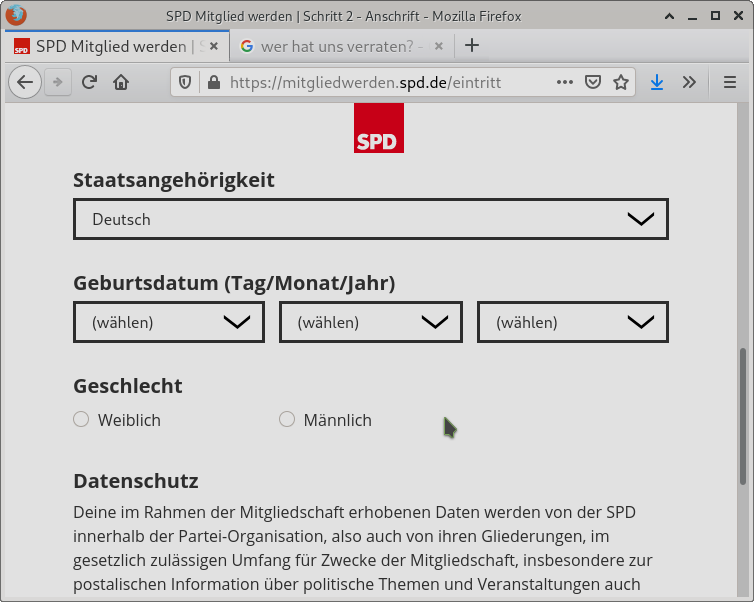
\includegraphics[scale=0.25,angle=0,keepaspectratio]{images/partei_spd.png}}
\pause
\Put(100,0){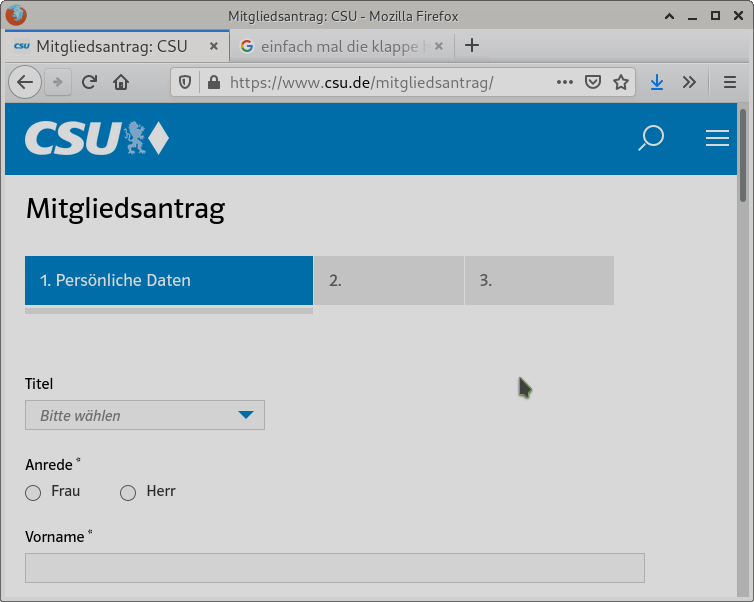
\includegraphics[scale=0.25,angle=5,keepaspectratio]{images/partei_csu.png}}
\pause
\Put(100,0){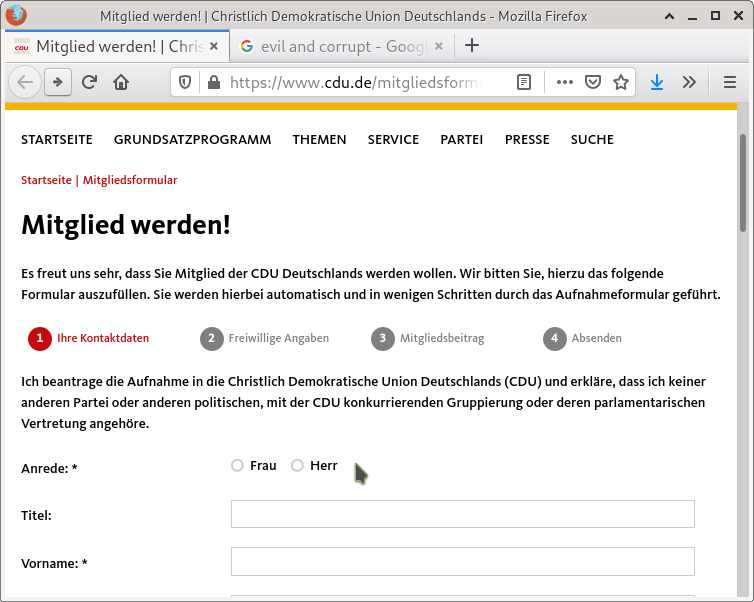
\includegraphics[scale=0.25,angle=-5,keepaspectratio]{images/partei_cdu.png}}
\pause
\Put(90,0){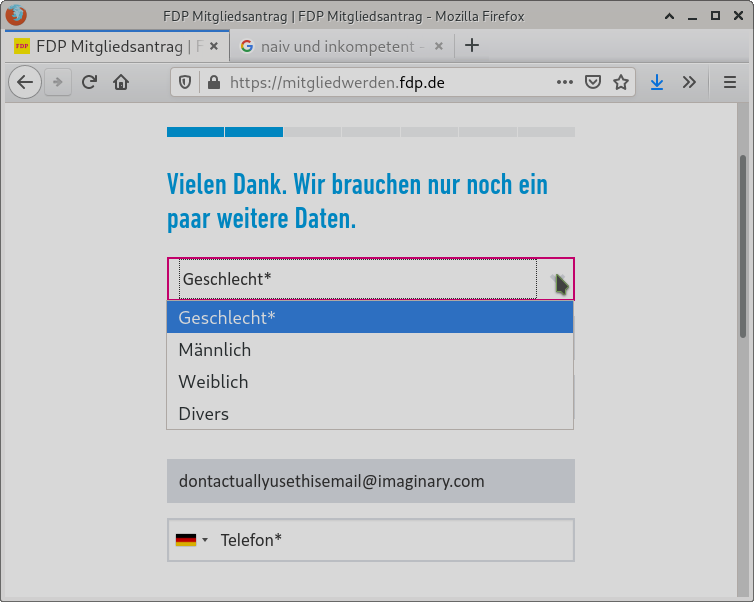
\includegraphics[scale=0.25,angle=10,keepaspectratio]{images/partei_fdp.png}}
\pause
\Put(90,0){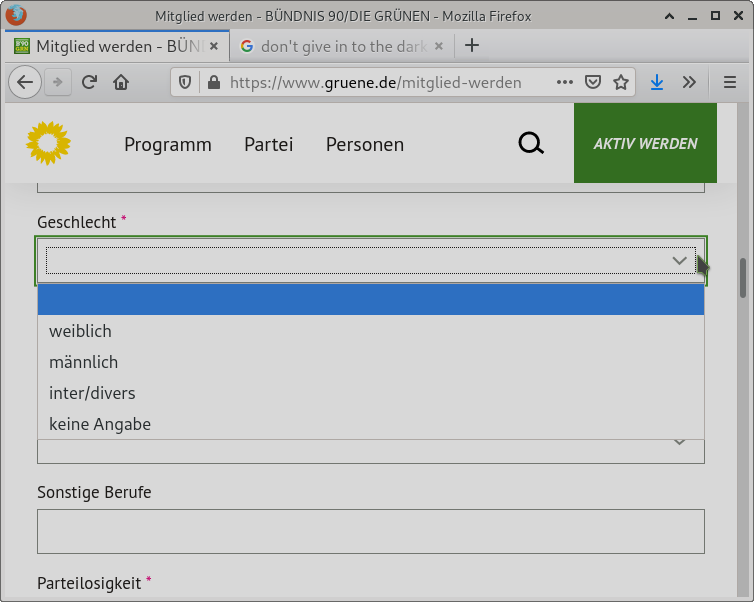
\includegraphics[scale=0.25,angle=-10,keepaspectratio]{images/partei_gruene.png}}
\pause
\Put(100,0){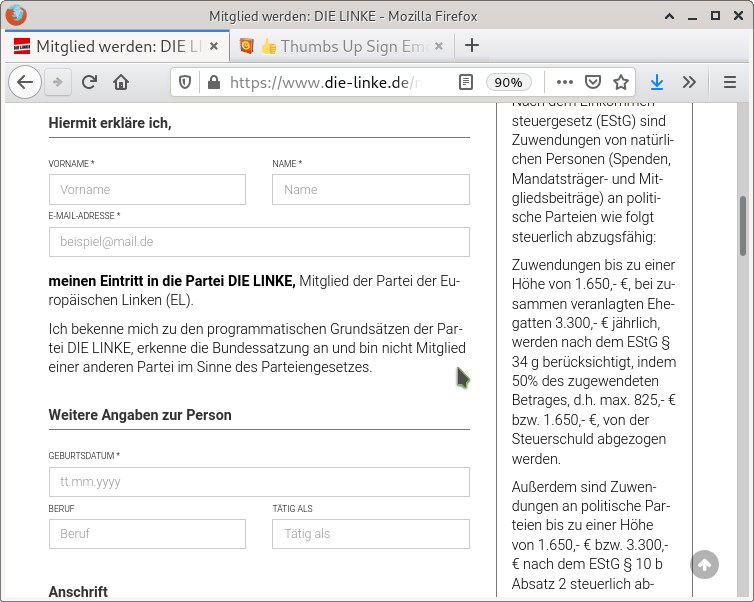
\includegraphics[scale=0.25,angle=0,keepaspectratio]{images/partei_linke.png}}
\Put(-20,0){
\includegraphics[scale=0.75]{images/party-popper.png}}
\Put(300,0){\reflectbox{
\includegraphics[scale=0.75]{images/party-popper.png}}}
\end{frame}

%------------------------------------------------------------------------------------

\section{How To Ask}

\begin{frame}
\begin{center}
\huge
No, but \emph{seriously}!\\
How \emph{do} I ask people for their\dots
\end{center}
\end{frame}

\begin{frame}
\frametitle{\dots Gender? \dots Orientation? \dots}
\large
Before asking:
\begin{itemize}
\item Make sure you \emph{need} the information.
\item Make sure \emph{this} is the information you need.
\item Make sure its \emph{mutable} in your model.
\item Make sure you \emph{understand} the question you're asking.
\end{itemize}
\bigskip

\emph{And then ask!} Tell them, what you need the answer for and give as many options as is reasonable under the circumstances (that's \emph{almost always} more than 2!) but also leave a text field for people who don't find themselves in those options.
\end{frame}

\begin{frame}
\frametitle{Popular with the Target Demographic}
\begin{center}
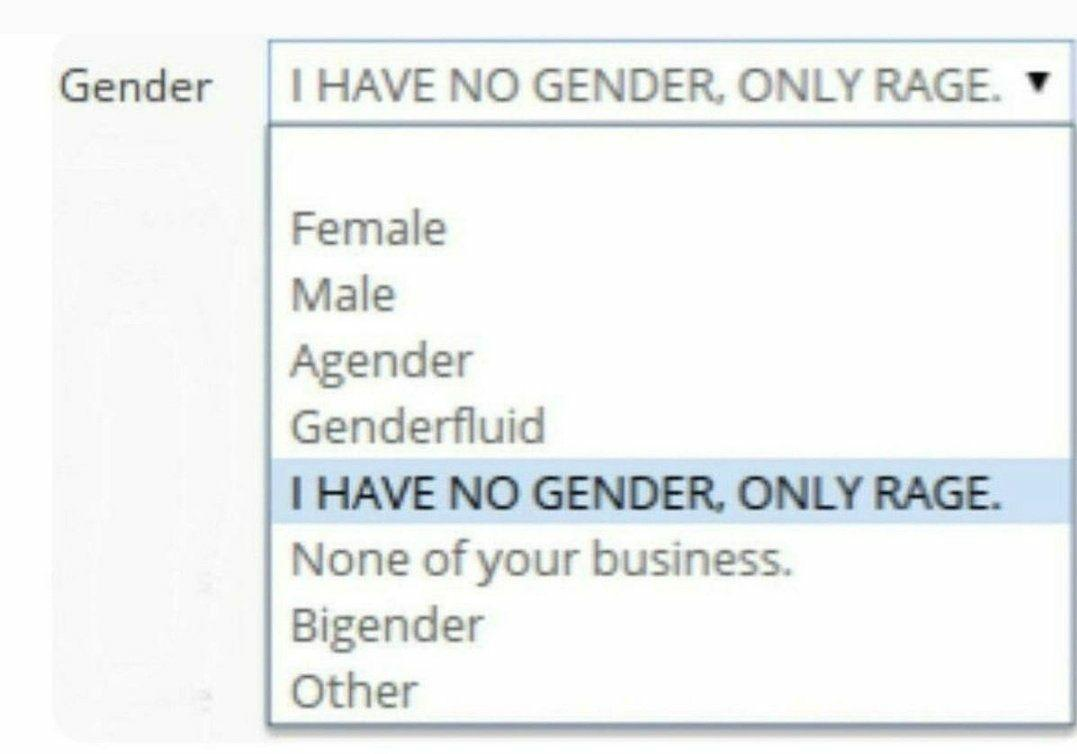
\includegraphics[height=0.725\textheight,keepaspectratio]{images/gender_RAGE.jpg} 
\end{center}
\end{frame}

\begin{frame}
\begin{center}
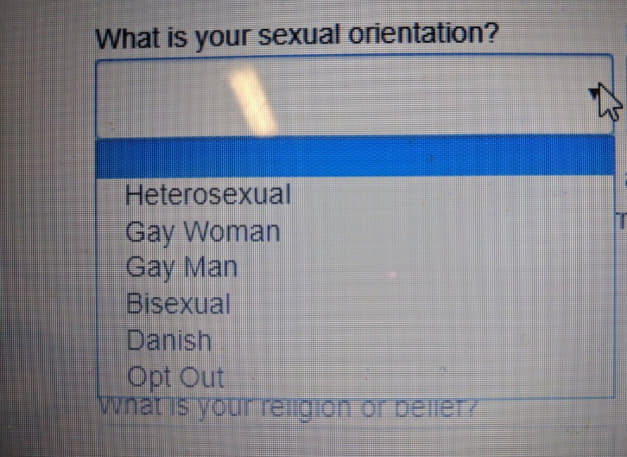
\includegraphics[height=0.8\textheight,keepaspectratio]{images/theashencouncil_01.png} 
\end{center}
\end{frame}

%------------------------------------------------------------------------------------

\section{End}

\begin{frame}
\frametitle{Future Work}

\begin{minipage}{0.5\textwidth}
\Large
Addresses:
\large
\end{minipage}\pause%
\begin{minipage}{0.5\textwidth}
\Large
Names:
\large
\end{minipage}
\pause\bigskip\large

\begin{center}
\dots but the way to deal with them is the same!
\end{center}

\end{frame}

\begin{frame}
\frametitle{Conclusion, again!}
\large
The central points of this talk are as follows:\bigskip

\begin{itemize}
\item \textbf{Make the model fit the user and not vice versa!}\\
\emph{All models are wrong, some are useful. Stereotypes aren't!}\medskip
\item \textbf{Humans are moving targets!}\\
\emph{Humans change all the time. Your model will have to change with them!}\medskip
\item \textbf{The empty model makes the fewest mistakes!}\\
\emph{You can't draw wrong conclusions from data you don't collect.}\medskip
\item \textbf{Precision and transparency are key!}\\
\emph{Make sure that both you and your users know what you're using the data for.}
\end{itemize}

\end{frame}

\begin{frame}
\frametitle{Recommendations:}
\small

\emph{``False assumptions developers make about gender''} by \href{https://twitter.com/ineffyble}{\texttt{@ineffyble}}\\
\scriptsize
\url{https://speakerdeck.com/ineffyble/false-assumptions-developers-make-about-gender-and-their-sometimes-hilarious-results}
\small\bigskip

\emph{Falsehoods programmers believe about}\dots
\begin{itemize}
\scriptsize
\item\dots gender:\\ \url{https://medium.com/gender-2-0/falsehoods-programmers-believe-about-gender-f9a3512b4c9c}
\item\dots names:\\ \url{https://shinesolutions.com/2018/01/08/falsehoods-programmers-believe-about-names-with-examples/}
\item\dots addresses:\\ \url{https://www.mjt.me.uk/posts/falsehoods-programmers-believe-about-addresses/}
\end{itemize}

\small
\emph{Geschickt Gendern -- Das Genderwörterbuch}: \url{https://geschicktgendern.de/}
\end{frame}

%------------------------------------------------------------------------------------

\end{document}

